% !TEX encoding = UTF-8 Unicode
\graphicspath{{figuras/}}

\chapter{Dicas do \LaTeX}
\label{cap2}

Dicas\footnote{Recomenda-se que todo capítulo seja iniciado com um parágrafo resumo introdutório do capítulo descrevendo o assunto e o escopo ou principais tópicos abordados.} de uso e exemplos de recursos do \LaTeX\ são apresentados. O \LaTeX\   é uma ferramenta poderosa para editar relatórios técnicos pois nos permite estruturar o conteúdo com citações e referências cruzadas para figuras, código de programa e equações de forma programática. Acrescentar ou modificar textos no \LaTeX\ é facilitado, pois figuras e listagens de códigos podem ser armazenadas em arquivos externos e incluídos facilmente no corpo do texto. As modificações feitas nas figuras ou códigos são automaticamente formatadas. Além disso, a ideia central do \LaTeX, \, que é baseada em macros, nos permite personalizar trechos de texto que se repetem ou que desejamos que possuam um comportamento predefinido. 

Para uma breve introdução ao \LaTeX\ recomenda-se o site  \url{https://www.overleaf.com/learn/latex/Learn_LaTeX_in_30_minutes}, que oferece uma conta gratuita para editar documentos  com o \LaTeX\ online. No \emph{Overleaf} você aprende \LaTeX\ sem precisar instalar nenhum aplicativo. Se preferir instalar um editor dedicado ao \LaTeX,\,  experimente  o \url{https://texstudio.org} que é gratuito e possui uma interface amigável. O TexStudio requer uma instalação \LaTeX\ como o \url{https://www.tug.org/texlive/}.

Quando precisar de ajuda ao encontrar algum erro de compilação em seu documento, use a máquina de busca do Google com a mensagem de erro. Um dos sites que sempre retorna com boas dicas é o [https://tex.stackexchange.com], que é o site que recomendo buscar por ajuda. 

Divirta-se!

\section{Por que \LaTeX?}
\LaTeX\ (pronunciado``Lei tec,'' ou ``La tec,'' jamais ``Lei tex'' ou ``Látex'') é um programa de composição tipográfica que é padrão para redação profissional de textos técnico-científicos e matemáticos. \LaTeX\ é um ambiente de composição tipográfica  estruturado  que utiliza \emph{macros} para facilitar a editoração eletrônica. 

\begin{example}[Definição e uso de uma macro para comentar textos]

A definição da macro \texttt{$\backslash$arb}, usada pelo autor para fazer anotações destacadas no documento, possui dois parâmetros opcionais \texttt{[1=NB:, 2=red]}.
\begin{lstlisting}[language={[Latex]Tex},frame=single,numbers =none]
	\newcommandx{\arb}[3][1=NB:, 2=red!50!gray]{ \color{#2} #1 #3 \color{black}}
\end{lstlisting}
O uso desta macro nos permite formatar recomendações como  
\arb{Leia este capítulo para captar algumas dicas úteis do \LaTeX.}
em diferentes partes do documento mantendo a uniformidade da formatação ajustada modificando os parâmetros de rótulo e cor, i.e. \verb|\uwave{\arb[ARB:][blue]{outra observação ilustrando comentários!}}.| para sinalizar tipos de comentários ou autor do comentário. \uwave{\arb[ARB:][blue]{outra observação ilustrando comentários!}}
\QEDA
\end{example}

O \TeX\,  e o \LaTeX\ são aplicativos gratuitos cujas funcionalidades são incrementadas por meio de pacotes (packages) contendo variadas macros escritas  por inúmeros usuários que compartilham livremente o código. Por exemplo, para desenhar diagramas esquemáticos de circuitos usamos o pacote \texttt{circuitikz}, que é acrescentado no preâmbulo de um documento escrevendo como ilustrado no Código~\ref{lst:LatexBasicoDoc}. No caso do pacote \texttt{circuitikz} carrega-se o pacote com as opções \texttt{[siunitx,american,RPvoltages]}.

\begin{lstlisting}[language={[Latex]Tex},frame=single,numbers =none, caption= {Estrutura básica de um documento \LaTeX.},label=lst:LatexBasicoDoc]
\documentclass[a4paper,11pt]{article}
%---- Carregando  pacotes
\usepackage[usenames]{color} %usado para  cores
\usepackage{amssymb} % símbolos matemáticos para editar equações
\usepackage{amsmath} % Complementa o amssymb
\usepackage[siunitx,american, RPvoltages]{circuitikz} % para desenhar circuitos 
\usepackage{physics} % para editar, matrizes e operadores diferenciais
\usepackage[portuges]{babel} % língua portuguesa
\usepackage{xargs} % para definir newcommand com argumentos extras
%%--- Definindo Macros -----------------------------------
\newcommandx{\arb}[3][1=NB:, 2=red!50!gray]{ \color{#2} #1 #3 \color{black}}
% Equações são referenciadas entre parentesis. 
% Então use \bref{eq:minhaEquacao} ao invés \ref{eq:minhaEq}
\newcommand{\bref}[1]{\mbox{(\ref{#1})}}
%--- Início do corpo do documento ------------------------
\begin{document}
	\title{Assunto e proposta}
	\author{Nome do Autor} % Modifique o nome do autor aqui
	\maketitle
	
	\section{Introdução}
	
	Este é um documento \LaTeX\ em que a beleza de uma 
	equação linda \bref{eq:linda} é apreciada matematicamente 
	e tipograficamente como segue:
	
	\begin{equation} \label{eq:linda}
		\text{e}^{j\,\pi}+1=0
	\end{equation}
	
	\section{Comentários Finais}
	Programar e editar  texto em  \LaTeX\ 
	é elegantemente simples.
\end{document}
\end{lstlisting}

As dicas a seguir ajudam não apenas a editar um texto \LaTeX\ com uma sintaxe mais limpa, mas também a editar equações, mencionar corretamente citações e organizar a inserção de figuras isoladas ou agrupadas, com ou sem legenda para o grupo.  A inclusão de listagens de códigos de programas também é usual e recomenda-se o uso do pacote \texttt{mcode.sty}\footnote{A versão modificada anexado a este gabarito  inclui os códigos de caracteres acentuados necessário para exibir corretamente comentários de programas fonte  em português}. 

\section{O jeito \LaTeX\ de editar texto}

De início, destacamos a parte mais importante de um texto técnico: mencionar os créditos a quem publicou anteriormente trabalhos técnicos que usamos diretamente no trabalho que descrevemos. A diferença entre plágio e pesquisa é exatamente sobre isso. Pesquisa e desenvolvimento são realizados  buscando em diversas fontes  informações, procedimentos, algoritmos, etc., \textbf{citando a fonte com clareza} e onde é  obtida. \textbf{Plágio} é aquilo que se copia de um único trabalho ou de alguns poucos, mas as referências são omitidas para se ocultar os verdadeiros autores. Plágio é crime, além de ser uma vergonha acadêmica e profissional que causa desonra e cerceamento explícito dos pares (colegas de profissão, de sociedades técnico-científicas, etc.).

\subsection{Citações e referências cruzadas} 

\paragraph{As citações de referências bibliográficas} fazem parte da essência do \LaTeX. Para citar um livro, e.g. vou citar um livro clássico mas difícil de ler e entender que é \cite{Astrom:1970} (\verb|\cite{Astrom:1970}|), e outro do mesmo autor também clássico e muito bom é \cite{Astrom:1997} (\verb|\cite{Astrom:1997}|). O livro considerado a bíblia da Eletrônica é \cite{Horowitz:1981307}, que é referenciado usando o código: \verb|\cite{Horowitz:1981307}|.  A descrição completa do rótulo da referência bibliográfica  \texttt{Horowitz:1981307} bem como das demais citações está registrado em um arquivo texto separado estruturado no formato conhecido como \emph{Bibtex}.  Todas as referências bibliográfica usadas neste documento estão na mesma pasta junto deste gabarito  nos arquivos de texto \verb|ref_books.bib| e \verb|MinhasReferencias.bib|. Recomenda-se o uso do aplicativo \cite{JabRef2021} para editar e organizar bancos de dados com as referências bibliográficas.  

Os arquivosm que são bancos de dados de referências, são inseridos no documento nas penúltimas linhas do arquivo \texttt{masterdoc.tex} como 

\begin{lstlisting}[language={[Latex]Tex},frame=single]
	\bibliographystyle{apalike} % estilo escolhido para formatar a bibliografia
	\bibliography{ref_books,MinhasReferencias} %arquivos bibtex (database)
	%% NÃO pode haver espaço entre os nomes dos databases acima!!! (:-/ 
\end{lstlisting}

Note também que, Notas de Aula, embora sejam geralmente de acesso restrito aos alunos de determinada disciplina,  devem ser citadas caso sejam  usadas como referência no desenvolvimento de suas atividades e.g \cite{BragaAR2019} e citações para este documento, que é também um gabarito de relatório técnico com algumas dicas \LaTeX\ e de elaboração de proposta de projetos (\cite{bragaAR2021}).

\paragraph{Referências cruzadas} são menções às partes (seções, páginas) ou objetos (figuras, tabelas e equações) internas do documento que alinhavam os elos (\emph{links} ou \emph{hyperlinks}) que caracterizam um texto técnico. Um texto técnico é um documento preparado para facilitar uma leitura não linear\footnote{%
	Textos literários como romances são escritos assumindo uma leitura sequencial ou linear dos capítulos, visando construir suspense e aventura durante a leitura. Não se deve ler, de partida, o capítulo final de um romance, pois isso estraga a surpresa da história.}, %
 em que a ordem de leitura das partes do texto é estabelecida pelo leitor de acordo com a informação que se busca e ao conhecimento prévio dos assuntos abordados.  \emph{Por exemplo, orientadores, supervisores e avaliadores membros de bancas examinadoras, primeiramente, leem o resumo, partes da introdução como justificativa e objetivos e saltam para as conclusões para verificar se o que foi  proposto foi efetivamente  alcançado}. Desta forma, constrói-se uma expectativa de como o autor do documento demonstra e ilustra os resultados obtidos no corpo principal do documento em que se descreve a metodologia, arranjos experimentais e de simulação e a análise dos resultados.

\subsection{Comentários}

Quando se desenvolve um programa é essencial inserir comentários que não são compilados mas que ajudam o autor a recordar os motivos daquela codificação. Arquivos fonte  \LaTeX\ incluem, entremeados no texto principal,  variados códigos que estruturam e formatam o texto. Portanto, é recomendado que o autor insira comentários explicativos para recordar a posteriori alguma explicação relevante. O \LaTeX\ usa o caractere ``\%''   para comentar uma linha. Nada é formatado à direita  do caractere ``\%'' numa linha.

\verb|$f(t)=\sin(\omega\, t)$. \% esta função delineia um sinal senoidal| 

resulta em $f(t)=\sin(\omega\, t)$. % esta é a função senoidal

O caractere de comentário de linha ``\%'' é também usado como um símbolo coringa  para eliminar espaços vazios e evitar erros de compilação quando tais espaços interferem na lógica implementada de formatação.

\subsection{Estilo de fontes para  destacar texto}

O destaque de um texto é consistentemente obtido usando  a macro de  \emph{ênfase} (\verb|\emph{ênfase}|), que automaticamente seleciona o estilo itálico ou romano (não-itálico) de acordo com o contexto. Quando deseja-se destacar  no texto usando sempre um mesmo estilo usa-se  o   \textbf{negrito} (\verb|\textbf{negrito}|),  \textit{itálico} (\verb|\textit{itálico}|) ou \underline{sublinhado} (\verb|\underline{sublinhado}|). Código fonte ou nomes de comandos e macros são normalmente formatados com o estilo \texttt{teletipo} (\verb|\texttt{teletipo}|).

No ambiente de formato matemático o \textbf{negrito}, $\mathbf{R}$, é obtido com a macro (\verb|\mathbf{R}|), ou \emph{blackboard bold}, $\mathbb{R}$ (\verb|\mathbb{R}|) usados normalmente para descrever conjuntos de números reais $\mathbb{R}$, inteiros $\mathbb{Z}$, complexos $\mathbb{C}$, etc. 

Quando se está em modo matemático e é preciso escrever texto com fonte romana usamos a macro \verb|\text|.  Por exemplo, ao descrever uma função linear por partes denominada \texttt{rampa} usamos o ambiente \verb|case|:

\begin{multicols}{2}
	\begin{equation*}
		r(x)= \begin{cases}
			2\,x & \text{se }  x \ge 0 \\
			0 & \text{se }  x < 0
		\end{cases}
	\end{equation*}
	\vfill\null 
	\columnbreak
\begin{lstlisting}[language={[Latex]Tex},frame=single]
\begin{equation*}
	r(x)= \begin{cases}
		2 \, x & \text{se }  x \ge 0 \\
		0      & \text{se }  x < 0
	\end{cases}
\end{equation*}
\end{lstlisting}
\end{multicols}

\subsection{Espaços e mudança de linha}

O \LaTeX\ ignora espaços extras e quebra de linha. Por exemplo, 
\begin{lstlisting}[language={[Latex]Tex},frame=single]
	Uma sentença    longa       cheia         de espaços e com quebra 
	de linha é formatada     sem     os espaços    extras.
\end{lstlisting}

\fbox{Uma sentença    longa       cheia         de espaços e com quebra 
	de linha é formatada     sem     os espaços    extras.}

Salta-se uma linha vazia completa para quebrar um parágrafo em  dois. Coloca-se \verb|\\| no final de uma linha para criar uma nova linha, mas sem iniciar um novo parágrafo.

Usa-se  \verb|\noindent| para impedir a indentação de um novo parágrafo.

\paragraph{Para inserir espaçamento horizontal no texto} usa-se as macros  \verb|\quad|, \verb|\qquad|,  que deixam um espaço horizontal de, respectivamente,  um \texttt{em} e dois \texttt{em}s. O ``\texttt{em}''  é uma fonte dependendo do comprimento, frequentemente tão largo quanto um \texttt{M} maiúsculo na fonte atual.
\verb|\hspace {<skip>}| é um comando de espaçamento horizontal geral, que especifica a  quantidade \texttt{<skip>} de espaço horizontal. \verb|\hspace*{<skip>}| é análogo, mas não desaparecerá em uma quebra de linha. \verb|\hfill| é equivalente a \verb|\hspace{\fill}|.

\verb|\,| e \verb|\!| deixam, respectivamente, um espaço fino e um negativo; \verb|\,| é usado para inserir um espaço que representa multiplicação quando omitimos o ponto e.g. a operação $z = x \cdot y$ (\verb|$z = x \cdot y$|) é simplificada inserindo um espaço entre as variáveis \verb|$z = x \, y$| que resulta em $z = x \, y$. A falta do caractere de espaço  \verb|\,| produz uma formatação não recomendada, e.g. \verb|$z = x  y$| que resulta em $z = x y$.

\paragraph{Para inserir espaçamento  vertical } usa-se \verb|\vspace{1 cm}|, em que \SI{1}{\centi\meter} é o tamanho do espaço desejado entre parágrafos. \verb|\vfill| é equivalente a \verb|\vspace{\fill}| e diz ao \TeX\ para preencher com espaços em branco.

\paragraph{As dimensões de comprimento} usadas no \LaTeX\ estão relacionadas na Tabela~\ref{tab:DimLatex}.

\begin{table}
	\caption{Dimensões de comprimento usadas pelo \LaTeX.}	\label{tab:DimLatex}
\begin{tblr}{ 
		hlines={gray!50},
		vlines={gray!50},
		column{1}   = {bg=azure5, fg=white, font=\sffamily},
		column{3}   = {bg=azure5, fg=white, font=\sffamily},
		row{1}   = {bg=azure3, fg=white, font=\sffamily},
		colspec={Q[2] Q[5] Q[2] Q[5]},
	}
	Abreviação & Descrição & Código \LaTeX\ & Descrição\\
	\num{1} pt  & $\approx \SI{0.35}{\milli\meter}$  & $\backslash$quad & $18$ \texttt{mu}\\
	\num{1} mm  & um milímetro  & $\backslash,$ & $3$ \texttt{mu}\\
	\num{1}  cm  & um centímetro & $\backslash:$ & $4$ \texttt{mu}\\
	\num{1}  in  & uma polegada $\approx\SI{2.54}{\centi\meter}$ & $\backslash;$ & $5$ \texttt{mu}\\
	\num{1} \texttt{ex} & aproximadamente a altura de um ``x'' minúsculo e depende sempre da fonte usada.& $\backslash!$ & $-3$ \texttt{mu}\\
	\num{1} \texttt{em} & aproximadamente a largura de um ``M'' maiúsculo e depende sempre da fonte usada.& $\backslash$\textvisiblespace & ``barra invertida-espaço'' equivale a um espaço normal do texto\\
	\num{1} \texttt{mu} & unidade matemática igual a $\frac{1}{18}$\texttt{em}, em que \texttt{em} depende da família de fonte matemática usada. & $\backslash$qquad & $36$ \texttt{mu}
\end{tblr}
\end{table}

\subsection{Listas}

Listas são editadas de duas maneiras: ordenada (\verb|enumerate|) ou não ordenada (\verb|itemize|). Em ambos os casos é importante manter o paralelismo de linguagem, i.e. se o item começar com um verbo, todos os demais devem ser verbos também. Se escolher um substantivo, mantenha todos os itens iniciando com substantivos. O nosso cérebro não aprecia quebra de paralelismo de linguagem em listas e  em enumerações no meio do texto também!

\begin{multicols}{2}
	As três etapas essenciais em um sistema de automação são:
	\begin{enumerate}
		\item Energizar
		\item Partir
		\item Parar
	\end{enumerate}
	\vfill\null 
	\columnbreak
	\begin{lstlisting}[language={[Latex]Tex},frame=single]
		As três etapas essenciais em um 
		sistema de automação são:
		\begin{enumerate}
			\item Energizar
			\item Partir
			\item Parar
		\end{enumerate}
	\end{lstlisting}
\end{multicols}
%		\vfill\null 
\begin{multicols}{2}
	Avaliamos para:
	\begin{itemize}
		\item Conhecer
		\item Valorizar
		\item Responsabilizar
	\end{itemize}
		\vfill\null 
	\columnbreak
	\begin{lstlisting}[language={[Latex]Tex},frame=single]
		Avaliamos para:
		\begin{itemize}
			\item Conhecer
			\item Valorizar
			\item Responsabilizar
		\end{itemize}
	\end{lstlisting}
\end{multicols}

\section{Diferenciando formatação para matemática, texto, operadores ou funções}
Em uma composição tipográfica matemática adequada, as variáveis aparecem em itálico (e.g., $ f(x)=a\, x^2+ b\,x+c$). A exceção a esta regra são os \textbf{operadores} e  as \textbf{funções} predefinidas (e.g. $ \sin(x) $). Portanto, é importante \uwave{sempre} tratar \emph{texto}, \emph{variáveis}, \emph{operadores} e \emph{funções} corretamente. Veja a diferença entre $x$ e x, -1 e $-1$, e $sin(x)$ e $\sin(x)$.

Há duas maneiras de apresentar uma expressão matemática --- \emph{inline} ou como um estilo destacado numa linha própria como \emph{equação}.

\subsection{Expressões matemáticas estilo \emph{inline}}
As expressões \emph{inline} são usadas como uma palavra no meio de uma frase. Para inserir uma expressão \emph{inline}, coloque a expressão matemática entre os cifrões (\verb|$|). Por exemplo, digitando 

\begin{lstlisting}[language={[Latex]Tex},frame=single,numbers =none]
	A representação polar de $ Z =10\, \phase{\ang{90}}$ na forma exponencial é
	 $ Z =10\,\text{e}^{j\, \frac{\pi}{2}}$.
\end{lstlisting}
resulta no texto formatado\footnote{As macros \texttt{$\backslash$phase{$\backslash$ang\{90\}}} são providas pelos pacotes \texttt{steinmetz} e \texttt{siunitx}, respectivamente.}

\fbox{A representação polar de $ Z =10\, \phase{\ang{90}}$ na forma exponencial é
	$ Z =10\,\text{e}^{j\, \frac{\pi}{2}}$.}


Note o uso da macro de espaço ``\verb|\,|'' entre o módulo e ângulo e módulo e a parcela exponencial para prover o espaçamento adequado que representa multiplicação.


\paragraph{\emph{Displaystyle}} Para obter expressões matemáticas \emph{inline} em tamanho real, use \verb|\displaystyle|. Não obstante, recomenda-se moderação neste uso. Digitando 

\begin{lstlisting}[language={[Latex]Tex},frame=single,numbers =none]
	O estilo em tamanho real de um valor  médio é  
	$\displaystyle \frac{1}{N}\sum_{k=1}^{N}x(k)$, ao invés de 
	 $\frac{1}{N}\sum_{k=1}^{N}x(k)$.
\end{lstlisting} 

resulta na seguinte formatação:
 
\fbox{O estilo em tamanho real de um valor  médio é  $\displaystyle \frac{1}{N}\sum_{k=1}^{N}x(k)$, ao invés de  $\frac{1}{N}\sum_{k=1}^{N}x(k)$.}

\subsection{Expressões matemáticas estilo \emph{equação}}
Equações são expressões matemáticas que possuem sua própria linha e são centralizadas na linha. Geralmente,  é usado para equações importantes que merecem ser apresentadas em sua própria linha ou para grandes equações que não cabem numa linha. 

Para produzir uma  expressão neste estilo conhecido como \emph{display}, coloque a expressão matemática entre os símbolos de\textbf{ cifrões duplos}, i.e. \verb|$$| e \verb|$$|. Equivalentemente e mais recomendado entre os símbolos \verb|\[| e \verb|\]|, pois esta última sintaxe é mais amigável para o aplicativo \LaTeX\ detectar o ambiente de estilo \emph{display}. 

Digitando  \verb|$$ x=\frac{-b\pm\sqrt{b^2-4\,a\,c}}{2\,a} $$| 

ou  \verb|\[x=\frac{-b\pm\sqrt{b^2-4\,a\,c}}{2\,a}\]| resulta em  \[x=\frac{-b\pm\sqrt{b^2-4\,a\,c}}{2\,a}.\]

Para editar equações que se deseja referenciar no texto, usa-se o ambiente \texttt{equation} com um rótulo (\texttt{label}) como segue:

\begin{lstlisting}[language={[Latex]Tex},frame=single,numbers =none]
	\begin{equation} \label{eq:piuBella}
		\frac{dy}{dt} = a \, y.   
	\end{equation}
\end{lstlisting} 
obtendo 
	\begin{equation} \label{eq:piuBella}
	\frac{dy}{dt} = a \,  y.   
\end{equation}
em que um rótulo ou \emph{label} é usado para referência cruzada, \verb|\bref{eq:piuBella}|, a uma equação que é bela \bref{eq:piuBella}. 

Para destacar a equação num parágrafo próprio sem numerá-la sequencialmente quando estiver usando o ambiente \texttt{equation}, usa-se um asterisco (*) como segue:
\begin{lstlisting}[language={[Latex]Tex},frame=single,numbers =none]
	\begin{equation*}
		\text{e}^{j\,\pi}+1=0.
	\end{equation*}
\end{lstlisting}

\begin{equation*}
	\text{e}^{j\,\pi}+1=0.
\end{equation*}


A referência a uma equação é feita usando numeração entre parênteses, e.g. a equação \bref{eq:piuBella} é uma das mais belas equações matemáticas.

Uma forma mais elegante de editar equações é usando o pacote \emph{physics} que resulta em uma equação com o operador derivada: \verb|$\dv{y}{t}$| para formatar $\dv{y}{t} = a \, y$ ou simplesmente   \verb|$\dd{t}$| para formatar $\dd{t}$, representado o operador derivada com fonte \emph{roman} (não-itálico). Os exemplos a seguir ilustram o uso destes operadores: 
\begin{align} \label{eq:piuBella2}
	\dv{y}{t} &= a \, y, \\  % note o uso do comando \, para inserir um pequeno espaço entre a e y.
	y &= \int \dv{y}{t} \dd{t}.   % note o uso do comando \, para inserir um pequeno espaço entre a e y.
\end{align}
Compare o operador diferencial ``d'' nas equações \bref{eq:piuBella} e  \bref{eq:piuBella2}.
Ao escrever a função exponencial, lembre-se de escrever a constante $\text{e}=2.71828\cdots$ usando o formato de texto não-itálico, \verb|$\text{e}^{-t/\tau}$| que produz: $\text{e}^{-t/\tau}$.


\subsubsection{ Índices, expoentes e caracteres delimitadores}

Índices e expoentes são \emph{sempre} representados no \textbf{modo matemático} usando os caracteres sublinhado (\emph{underscore}) ``\_{}'' e circunflexo ``\^{}'', e.g. \verb|$x_1$|, \verb|$x^2$| que resultam em $x_1$, $x^2$.


\begin{tabular}{lllll}
	\toprule
	\emph{Descrição} & \emph{Comando}  & \emph{Resultado} &\emph{Objetos grandes} & \emph{Resultado}\\
	\midrule
	Parêntesis &\verb|(x)| & (x) &\verb|$\qty(\dfrac{1}{\tau\, s})$| & $\qty(\dfrac{1}{\tau\, s})$\\
	Colchetes &\verb|[x]| & [x]&\verb|$\qty[\dfrac{1}{\tau\, s}]$| & $\qty[\dfrac{1}{\tau\, s}]$\\
	Chaves & \verb|\{x\}| & \{x\}&\verb|$\qty{\dfrac{1}{\tau\, s}}$$| & $\qty{\dfrac{1}{\tau\, s}}$\\
	\bottomrule
\end{tabular}

Para tornar os delimitadores grandes o suficiente para abraçar o conteúdo, use-os junto com \verb|\right| e \verb|\left|. Usando o pacote \texttt{physics},  a macro \verb|\qty()| formata corretamente objetos de qualquer tamanho, simplificando a edição.

O par de chaves $\qty{}$ é um par de caracteres invisíveis quando formatados. Eles são usados para agrupar texto e objetos formados por mais de um caractere. Observe as diferenças nas seguintes expressões
\verb|$x^2$ e $x^{2}$| que produzem o mesmo resultado $x^2$ e $x^{2}$; mas \verb|$x^2t$ e $x^{2t}$| produzem resultados diferentes $x^2t$ e $x^{2t}$. O mesmo ocorre quando usamos índices e expoentes   \verb|$x_a^2$, $x_ab^2$, $x_{ab}^2$|, que resulta em $x_a^2$, $x_ab^2$ ,$x_{ab}^2$. Expoentes compostos por frações requerem o par de chaves $\qty{}$ para delimitar corretamente o grupo do expoente, e.g. \verb|$x_1^{-\frac{1}{2}}$| que produz $x_1^{-\frac{1}{2}}$. No caso de objetos grandes, recomenda-se o uso da macro \verb|\qty()| para redimensionar a altura de parêntesis, colchetes ou chaves, pois simplifica a edição consideravelmente, e.g.

\begin{lstlisting}[language={[Latex]Tex},frame=single,numbers =none]
$G(x,m,s)=\frac{1}{s\sqrt{2\pi}}\text{e}^{-\frac{1}{2}\,\qty(\frac{x-m}{s})^2}.$
\end{lstlisting} 
resulta em $\boxed{G(x,m,s)=\frac{1}{s\sqrt{2\pi}}\text{e}^{-\frac{1}{2}\,\qty(\frac{x-m}{s})^2}.}$

\subsubsection{Arranjos e Matrizes}
Para inserir matrizes  uma codificação usual é como segue:
\begin{lstlisting}[language={[Latex]Tex},frame=single,numbers =none]
$D = \begin{bmatrix} 
	 1  &   0 & 0\\
	-1  &   1 & 0\\
	 0  &  -1 & 1
	\end{bmatrix}$, 
% você pode escrever tudo em uma linha pois a quebra de linha é feita com "\\"
$S = \begin{bmatrix} 1  & 0  &  0\\ 1  & 1  & 0\\ 1  & 1  & 1 \end{bmatrix}$,
$x = \begin{bmatrix}  3\\  1\\  9 \end{bmatrix}$,   
$Dx = \begin{bmatrix} 3\\ -2\\  8 \end{bmatrix}$, 
$Sx = \begin{bmatrix} 3\\  4\\ 13 \end{bmatrix}$
\end{lstlisting}

que resulta em

$D = \begin{bmatrix} 
	1   &  0 &    0\\
	-1   &  1&     0\\
	0   & -1 &    1
\end{bmatrix}$, 
% você pode escrever tudo em um linha lembrando de usar a quebra de linha no modo matemático "\\"
$ S = \begin{bmatrix} 1    & 0   &  0\\ 1    & 1   &  0\\ 1   &  1   &  1 \end{bmatrix}$,
$x = \begin{bmatrix} 3\\ 1\\ 9 \end{bmatrix}$,   $Dx = \begin{bmatrix} 3\\ -2\\8 \end{bmatrix}$, $Sx = \begin{bmatrix} 3\\ 4\\ 13 \end{bmatrix}$

Todavia, usando o pacote \texttt{physics} fica mais  fácil e limpo a codificação:
\begin{lstlisting}[language={[Latex]Tex},frame=single]
	$D = \bmqty{1 & 0 &  0\\ -1  & 1 &  0\\ 0 & -1 & 1}$, 
	$S = \bmqty{1 & 0 &  0\\  1  & 1 &  0\\ 1 &  1 & 1}$, 
	$x = \bmqty{  3\\  1\\  9}$,   
	$Dx = \bmqty{ 3\\ -2\\  8}$, 
	$Sx = \bmqty{ 3\\  4\\ 13}$.
\end{lstlisting}

que resulta em 
$D = \bmqty{1   &  0 &    0\\-1   &  1&     0\\0   & -1 &    1}$, $ S = \bmqty{ 1    & 0   &  0\\ 1    & 1   &  0\\ 1   &  1   &  1 }$, $x = \bmqty{ 3\\ 1\\ 9 }$,   $Dx = \bmqty{ 3 \\ -2 \\ 8 }$, $Sx = \bmqty{ 3\\ 4\\ 13 }$.


Se quiser apresentar uma matriz de forma adensada, o pacote \texttt{physics} tem o comando 
\begin{verbatim}
	$ S = \sbmqty{ a  & b  \\ c  & d   }$
\end{verbatim}
que produz $ S = \sbmqty{ a  & b  \\ c  & d   }$.

O pacote \texttt{physics} também cria uma sintaxe elegante para digitar funções como seno e cosseno.
A equação $\sin[2](\theta) + \cos[2](\theta)=1$ é digitada usando o pacote \texttt{physics}\footnote{
	Para entender as demais macros do pacote \texttt{physics}, leia o manual  \texttt{https://ctan.org/pkg/physics?lang=en}.} como
\begin{verbatim}
	$\sin[2](\theta) + \cos[2](\theta)=1$.
\end{verbatim}

Uma equação é facilmente editada com índices:
\begin{verbatim}
	\begin{equation}\label{eq:QuedaVoltagem}
		V_{AB} = V_A - V_B. 
	\end{equation}
\end{verbatim}

que processado pelo \LaTeX\ resulta em
\begin{equation}\label{eq:QuedaVoltagem}
	V_{AB} = V_A - V_B. 
\end{equation}

Para escrever  somatórios e potência de variáveis usamos como exemplo a expressão de desvio padrão: 
\begin{lstlisting}[language={[Latex]Tex},frame=single]
	\begin{equation} \label{eq:desvioPadrao}
		s_x =\sqrt{\frac{1}{N-1}\sum_{k=1}^{N} \qty(x_k - \bar{x})^2},
	\end{equation}
\end{lstlisting}

Que resulta em:
\begin{equation}\label{eq:desvioPadrao}
	s_x =\sqrt{\frac{1}{N-1}\sum_{k=1}^{N} \qty(x_k - \bar{x})^2},
\end{equation}
em que $\bar{x}=\frac{1}{N}\sum_{k=1}^{N}x_k$ representa a média dos valores $x_k$. Observe como se pontua uma equação com vírgula \bref{eq:desvioPadrao} e ponto final \bref{eq:QuedaVoltagem}. Note o uso do comando \texttt{bref\{\}} para referenciar equações. O comando \texttt{bref\{\}}  está definido no preâmbulo do masterdoc.tex como
\begin{verbatim}
	\newcommand{\bref}[1]{\mbox{(\ref{#1})}}
\end{verbatim}
É simplesmente  uma macro usada para facilitar referência às equações sem esquecer de envolver o número de referência entre parêntesis. 

\section{Figuras}

Figuras são importantes  para ilustrar com fotos locais e arranjos experimentais, com diagramas  algum objeto, conceito, procedimento e, graficamente, resultados experimentais e dados. Considerando o ditado popular, \emph{uma imagem vale mais que mil palavras},  figuras normalmente  ocupam um espaço de parágrafo destacado do texto ou, mais raramente, envolvidas no meio do texto. Todavia, não basta simplesmente inserir figuras no documento, é imprescindível que toda figura inserida seja referenciada e comentada no corpo do texto, além de ser sucintamente descrita numa legenda própria. Para nos referirmos a uma figura posteriormente, toda figura tem que ser identificada com um rótulo ou \emph{label}.
As referências a um figura  são feitas identificando-se o objeto referenciado como {\emph{Figura} ou \emph{Fig. } seguido do caracter \verb|~| (\emph{nonbreaking space}) e de uma referência numérica \textit{sem parênteses}. 
A linha a seguir:

\begin{verbatim}
 O Diagrama de Blocos mostrado na  Figura~\ref{fig:MBPCauditor} 
 ilustra  uma arquitetura (...)
\end{verbatim}

resulta no seguinte texto formatado:

\fbox{O Diagrama de Blocos mostrado na  Figura~\ref{fig:MBPCauditor} ilustra uma arquitetura(...)}


O  modo tradicional para inserir figuras é feito usando o código  mostrado  no Programa~\ref{lst:IncludeFigura}.

\begin{lstlisting}[language={[Latex]Tex},frame=single,numbers =none, caption= {Sintaxe clássica para inserir uma figura.},label=lst:IncludeFigura]
\begin{figure}[!htbp]
	\centering
	\includegraphics[width=15cm]{MBPCauditor} 
	\caption{Arquitetura simplificada de um sistema de controle baseado em 
		modelo 	com a função de Auditor de Processo. Se desejar inserir 
		referência cruzada na legenda, lembre-se de proteger o comando com 
		\emph{protect}: Uma figura que se liga a uma bela 
		equação \protect\bref{eq:piuBella}.}
	\label{fig:MBPCauditor}
\end{figure}
\end{lstlisting}

Os parâmetros \verb|[!htbp]| indicam a sequência de prioridade para posicionar a figura: \textsf{h} here (aqui!), \textsf{t} top (no topo da página), \textsf{b} bottom (na parte inferior da página) e \textsf{p} page (numa página só de figuras).
%--- inseção de figura usando includegraphics{}--------
\begin{figure}[!htbp]
	\centering
	\includegraphics[width=12cm]{MBPCauditor} 
	\caption{Arquitetura simplificada de um sistema de controle baseado em modelo com a função de Auditor de Processo. Se desejar inserir referência cruzada na legenda, lembre-se de proteger o comando com \emph{protect}: Uma figura que se liga a uma bela equação \protect\bref{eq:piuBella}.}
	\label{fig:MBPCauditor}
\end{figure}
% ---------------------------------------------------------
Frequentemente, desejamos  inserir duas imagens ou gráficos agrupados numa mesma figura como sendo subfiguras. Estas figuras com múltiplos conteúdos podem ser identificadas com legendas para cada subfigura, com ou sem legenda única para a figura toda.  A inserção de figuras múltiplas é facilitada pelo pacote \verb|\usepackage{keyfloat}|. Além de simplificar a sintaxe de inserção de figuras, o pacote \verb|keyfloat| provê parâmetros e ambientes para agrupar figuras, tabelas e textos arranjados matricialmente\footnote{O pacote \emph{keyfloat} tem sido atualizado enquanto que os pacotes \emph{subfig} e \emph{subfigure} já são considerados obsoletos pela incompatibilidade com hyperlinks em arquivos $*.pdf$.}.

A sintaxe simplificada para inserir uma figura de um arquivo de imagem (\texttt{.pdf, .svg, .eps, .png,.jpg, .jpeg}) é
\begin{lstlisting}[language={[Latex]Tex},frame=single]
\keyfig{lw=0.75, c={Arquitetura simplificada de um sistema de controle.},
	l=fig:MBPCauditor2}{MBPCauditor.png}
 \end{lstlisting}

O parâmetro \texttt{lw=0.75} especifica o tamanho da figura em relação a largura da linha (\texttt{linewidth}). Os outros parâmetros  especificam a legenda (\emph{caption}) \texttt{c=\{Texto da legenda\}} e o rótulo da figura (\emph{label}) \texttt{l=fig:MBPCauditor2}.

\keyfig{lw=0.75, c={Arquitetura simplificada de um sistema de controle.},
	l=fig:MBPCauditor2}{MBPCauditor.png}

Para inserirmos uma figura com conteúdo variado diferente de um arquivo de imagem, e.g. o código de uma figura do \emph{CircuiTikz}, usamos a macro \texttt{$\backslash$keyfigbox} que cria uma figura com uma caixa de conteúdo arbitrário, em vez de uma imagem de um arquivo. Sua largura padrão é a largura de linha, a menos que os parâmetros (\emph{keys}) \texttt{w} ou \texttt{lw } sejam usados.
\begin{lstlisting}[language={[Latex]Tex},frame=single,numbers =none]
\keyfigbox{lw=1, c={Diagrama em blocos de uma cadeia de amostragem de um
sinal com um filtro anti-aliasing  analógico e um filtro anti-aliasing digital 
seguido por uma decimação de dados.}, l=fig:DBlocosFiltroAmostragemDecimador}{%
	%%------------------------------------------------------------------- %%
%	fig:DBlocosFiltroAmostragemDecimador
% Diagrama em blocos de uma cadeia de amostragem de um sinal 
% com um filtro anti-aliasing  analógico e um filtro 
% anti-aliasing digital seguido por uma decimação de dados
%
%  --- Anisio R. Braga, COLTEC-UFMG
%  --- 2021/01/25
%---------------------------------------------------------------------

\tikzset{
	alias path picture bounding box/.code=%
	\pgfnodealias{#1}{path picture bounding box},
	CNTRL/.style =
	{
		> = latex, % Triangle,
		block/.style = {rectangle, draw, thick,
			minimum height=12mm, minimum width=12mm,
			outer sep = 0mm},
		dot/.style = {fill,
			circle, inner sep=0mm, outer sep=0mm, minimum size=1mm,
			node contents={}},
		gain/.style = {thick, regular polygon, regular polygon sides=3, shape border rotate=-90, draw,
			inner sep=3pt, anchor=west, outer sep = 0mm},
		sum/.style = {circle, draw, thick, minimum size=6mm,
			path picture={%
				\tikzset{alias path picture bounding box=@}
				\draw[very thick, shorten <=1mm, shorten >=1mm, -]
				(@.north) edge (@.south)
				(@.west)   --  (@.east);
			},% end of node contents
			node contents={}},
	}% end of CNTRL style
}% end of tikzset
%-----------------------------

\begin{circuitikz}[CNTRL, node distance = 10mm and 10mm]
	\ctikzset{bipoles/oscope/width=1.2, bipoles/oscope/height=0.85} 
	\tikzstyle{bkgbox}=[draw, rectangle, inner sep=25pt, densely dotted, rounded corners=1mm, 
	teal, color=teal!50!gray,thick, fill=teal!5]
	% --- rand function seed
	\pgfmathsetseed{2.7}
	
	% --- Posicionando os blocos 
	% --- Bloco de entrada
	\node [block,fill=white] (Sensor) at (0,0){};
	\node at (Sensor.east) [above right] {\color{azul}$y_s$}; 
	\node[font=\small,below of=Sensor,label={[yshift=-0.5cm,align=center,font=\footnotesize]above: Sensor}]{};
	% sinal analógico do sensor
	\begin{scope}[shift={($(Sensor)+(-0.5,-0.375)$)},scale=0.65]
		\draw [gray, ->] (0,0) \coord(f3)  -- ++(1.6,0) node[below=-2pt,font=\tiny](){$t$};
		\draw [gray, ->] (f3)  -- ++(0,1.25);
		\draw[azul,thick, samples=50,domain=0:1.4] plot(\x,{0.8+0.65*exp(-1.5*\x)*sin(6*(\x+0.55) r)});  
	\end{scope}
	%--- Somador ruído
	\node (s1) [sum, right=of Sensor, node distance = 8mm ] {};
	\node at (s1.west) [above left] {$+$} ;
	\node at (s1.north) [above left, font=\footnotesize] {$+$};
	
	%--- Ruido
	\node (Ruido) [block,fill=white, above of =s1,node distance=1.5cm] {}; 
	\node[font=\scriptsize,left of = Ruido, align=center,node distance=1.1cm]{Ruído};
	\node at (Ruido.south) [below right, font=\footnotesize] {$\xi$};
	% sinal
	\begin{scope}[shift={($(Ruido)+(-0.6,-0.4)$)},scale=0.75]
		\begin{axis}[x=0.1cm,y=1cm,axis line style={draw=none},tick style={draw=none},xtick=\empty,ytick=\empty,
			samples=50,domain=0:13]
			\addplot[gray,thin, opacity=1] plot (\x, {0.5*rand});
		\end{axis}
	\end{scope}  
	%--- Filtro anti-aliasing analógico
	\node (FPB) [fill=white,block,right of=s1,node distance=2cm]  {$\dfrac{1}{\tau \, s+1}$}; 
	\node[below of=FPB,label={[yshift=-0.75cm,align=center,font=\footnotesize]above: Filtro Analógico\\ Anti-aliasing}]{};
	
	%--- ADC amostrador
	\node (ADC) [fill=white,block,right of=FPB,node distance=2.25cm] {}; 
	\draw ($(ADC)+(-0.5,0)$) to[spst, a=\small $h$]  ++(1,0); 
	\node at (ADC) [label={[yshift=0.5cm,align=center,font=\footnotesize]above: $\color{laranja}h=\tau$}]{};
	\node[font=\scriptsize,below of=ADC,label={[yshift=-0.75cm,align=center,font=\scriptsize]above: ADC \\ Amostrador}]{};
	%--- Filtro anti-aliasing digital
	\node (FPBd) [fill=white,block,right of=ADC,node distance=2.5cm]  {$\dfrac{(1-\beta) z^{-1}}{1-\beta z^{-1}}$};\  
	\node[below of=FPBd,label={[yshift=-0.75cm,align=center,font=\footnotesize]above: Filtro Digital \\ Anti-aliasing}]{}; 
	\node at (FPBd) [label={[yshift=0.5cm,align=left,font=\footnotesize]above: $\tau_f=m\,\color{laranja}h$\\ $\beta \approx \frac{2\,m-1}{2\,m+1}$}]{};
	%--- Decimador 
	\node (DEC) [fill=white,block,right of=FPBd,node distance=2.5cm] {}; % {\Ztransf}; 
	\draw ($(DEC)+(-0.5,0)$) to[spst, a=\small $h_1$ ]  ++(1,0); 
	\node at (DEC) [label={[yshift=0.5cm,align=center,font=\footnotesize]above: $\color{red!50!gray}h_1 \color{black}=m\,\color{laranja}h$}]{};
	\node[font=\scriptsize,below of=DEC,label={[yshift=-0.45cm,align=center,font=\footnotesize]above: Decimador}]{};
	%--- Controlador 
	\node (CTR) [fill=white,block,right of=DEC,node distance=2.2cm]  {$C(z^{-1})$}; 
	\node[below of=CTR,label={[yshift=-0.75cm,align=center,font=\footnotesize]above: Controlador\\ Digital}]{};
	%--- conexões
	\draw[->] (Sensor) -- (s1);   
	\draw[->] (Ruido) -- (s1.north); 
	\draw[->] (s1.east) -- (FPB);  
	\draw[->] (FPB) -- (ADC);  
	\draw[->] (ADC) -- (FPBd);  
	\draw[->] (FPBd) -- (DEC);  
	\draw[->] (DEC) -- (CTR);  
	%-----------------------------------
	%-----------------------------------------
	% desenhando esboço de gráficos dos sinais 
	%---- Saída analógica y
	\begin{scope}[shift={(-0.5,2.5)}]
		\draw [gray, ->] (0,0) \coord(f3)  -- ++(1.6,0) node[below=-2pt,font=\scriptsize](){$t$};
		\draw [gray, ->] (f3)  -- ++(0,1.25);
		\draw[azul,thick, samples=50,domain=0:1.4] plot(\x,{0.8+0.65*exp(-1.5*\x)*sin(6*(\x+0.55) r)});
		\draw[gray,-Stealth] [out=-90, in=90] (0.5,-0.15) to ($(Sensor.east)+(0.45,0.25)$); 
	\end{scope} 
	%---- Saída analógica y + ruido
	\begin{scope}[shift={(2,2.5)}]
		\draw [gray, ->] (0,0) \coord(f3)  -- ++(1.6,0) node[below=-2pt,font=\scriptsize](){$t$};
		\draw [gray, ->] (f3)  -- ++(0,1.25);
		\draw[azul, samples=70,domain=0:1.4] plot(\x,{0.2*rand+0.8+0.65*exp(-1.5*\x)*sin(6*(\x+0.55) r)});  
		\draw[gray,-Stealth] [out=-90, in=90]  (0.75,-0.15) to ($(s1.east)+(0.45,0.15)$) node[ label={below :\color{azul}{\small $y_s+\xi$}}]{};
	\end{scope} 
	
	%---- Saída analógica filtrada
	\begin{scope}[shift={(4.25,2.5)}]
		\draw [gray, ->] (0,0) \coord(f3)  -- ++(1.6,0) node[below=-2pt,font=\scriptsize](){$t$};
		\draw [gray, ->] (f3)  -- ++(0,1.25);
		\draw[laranja,semithick, smooth, samples=70,domain=0:1.4] plot(\x,{0.05*rand+0.8+0.65*exp(-1.5*\x)*sin(6*(\x+0.55) r)}); 
		\draw[gray,-Stealth] [out=-90, in=90] (0.5,-0.15) to ($(FPB.east)+(0.45,0.15)$)node[ label={below :\color{laranja}{\small $y(t)$}}]{}; 
	\end{scope} 
	
	%--- Saída ADC amostrador
	\begin{scope}[shift={(6.75,2.5)}]
		\draw [gray, ->] (0,0) \coord(f3)  -- ++(1.65,0) node[below=-2pt,font=\scriptsize](){$k\,h$};
		\draw [gray, ->] (f3)  -- ++(0,1.2);
		\draw[ycomb, mark=*, mark size=1.25pt,samples=14,domain=0:1.4] plot(\x,{0.05*rand+0.8+0.65*exp(-1.5*\x)*sin(6*(\x+0.55) r)});	
		\draw[gray,-Stealth]  (0.75,-0.15) to[out=-90, in=90] ($(ADC.east)+(0.45,0.15)$) node[ label={below :\color{black}{\small $\breve{y}(k)$}}]{};
	\end{scope}
	
	%--- Saída FPBd decimador
	\begin{scope}[shift={(9.25,2.5)}]
		\draw [gray, ->] (0,0) \coord(f3)  -- ++(1.65,0) node[below=-2pt,font=\scriptsize](){$k\,h$};
		\draw [gray, ->] (f3)  -- ++(0,1.2);
		\draw[red!50!gray,smooth, ycomb, mark=*, mark size=1.25pt,samples=14,domain=0:1.4] plot(\x,{0.8+0.6*exp(-1.5*\x)*sin(6*(\x+0.6) r)});  
		\draw[gray,-Stealth] (0.75,-0.15) to[out=-80, in=100] ($(FPBd.east)+(0.45,0.15)$) node[ label={below :\color{red!50!gray}{\small $\hat{y}_f(k)$}}]{};
	\end{scope}
	%--- Saída Decimador
	\begin{scope}[shift={(11.75,2.5)}]
		\draw [gray, ->] (0,0) \coord(f3)  -- ++(1.65,0) node[below=-2pt,font=\scriptsize](){$k\,h_1$};
		\draw [gray, ->] (f3)  -- ++(0,1.2);
		\draw[ycomb, mark=*, mark size=1.25pt,samples=7,domain=0:1.4] plot(\x,{0.8+0.6*exp(-1.5*\x)*sin(6*(\x+0.6) r)});  
		\draw[gray,-Stealth]  (0.75,-0.15) to[out=-90, in=90] ($(DEC.east)+(0.45,0.15)$) node[ label={below :\color{black}{\small $\hat{\hat{y}}_f(k)$}}]{};
	\end{scope}
	
	%-------------------------------------------------
\end{circuitikz}

}
\end{lstlisting}

\keyfigbox{lw=1, c={Diagrama em blocos de uma cadeia de amostragem de um
		 sinal com um filtro anti-aliasing  analógico e um filtro anti-aliasing digital 
		 seguido por uma decimação de dados.},	l=fig:DBlocosFiltroAmostragemDecimador}{%
	%%------------------------------------------------------------------- %%
%	fig:DBlocosFiltroAmostragemDecimador
% Diagrama em blocos de uma cadeia de amostragem de um sinal 
% com um filtro anti-aliasing  analógico e um filtro 
% anti-aliasing digital seguido por uma decimação de dados
%
%  --- Anisio R. Braga, COLTEC-UFMG
%  --- 2021/01/25
%---------------------------------------------------------------------

\tikzset{
	alias path picture bounding box/.code=%
	\pgfnodealias{#1}{path picture bounding box},
	CNTRL/.style =
	{
		> = latex, % Triangle,
		block/.style = {rectangle, draw, thick,
			minimum height=12mm, minimum width=12mm,
			outer sep = 0mm},
		dot/.style = {fill,
			circle, inner sep=0mm, outer sep=0mm, minimum size=1mm,
			node contents={}},
		gain/.style = {thick, regular polygon, regular polygon sides=3, shape border rotate=-90, draw,
			inner sep=3pt, anchor=west, outer sep = 0mm},
		sum/.style = {circle, draw, thick, minimum size=6mm,
			path picture={%
				\tikzset{alias path picture bounding box=@}
				\draw[very thick, shorten <=1mm, shorten >=1mm, -]
				(@.north) edge (@.south)
				(@.west)   --  (@.east);
			},% end of node contents
			node contents={}},
	}% end of CNTRL style
}% end of tikzset
%-----------------------------

\begin{circuitikz}[CNTRL, node distance = 10mm and 10mm]
	\ctikzset{bipoles/oscope/width=1.2, bipoles/oscope/height=0.85} 
	\tikzstyle{bkgbox}=[draw, rectangle, inner sep=25pt, densely dotted, rounded corners=1mm, 
	teal, color=teal!50!gray,thick, fill=teal!5]
	% --- rand function seed
	\pgfmathsetseed{2.7}
	
	% --- Posicionando os blocos 
	% --- Bloco de entrada
	\node [block,fill=white] (Sensor) at (0,0){};
	\node at (Sensor.east) [above right] {\color{azul}$y_s$}; 
	\node[font=\small,below of=Sensor,label={[yshift=-0.5cm,align=center,font=\footnotesize]above: Sensor}]{};
	% sinal analógico do sensor
	\begin{scope}[shift={($(Sensor)+(-0.5,-0.375)$)},scale=0.65]
		\draw [gray, ->] (0,0) \coord(f3)  -- ++(1.6,0) node[below=-2pt,font=\tiny](){$t$};
		\draw [gray, ->] (f3)  -- ++(0,1.25);
		\draw[azul,thick, samples=50,domain=0:1.4] plot(\x,{0.8+0.65*exp(-1.5*\x)*sin(6*(\x+0.55) r)});  
	\end{scope}
	%--- Somador ruído
	\node (s1) [sum, right=of Sensor, node distance = 8mm ] {};
	\node at (s1.west) [above left] {$+$} ;
	\node at (s1.north) [above left, font=\footnotesize] {$+$};
	
	%--- Ruido
	\node (Ruido) [block,fill=white, above of =s1,node distance=1.5cm] {}; 
	\node[font=\scriptsize,left of = Ruido, align=center,node distance=1.1cm]{Ruído};
	\node at (Ruido.south) [below right, font=\footnotesize] {$\xi$};
	% sinal
	\begin{scope}[shift={($(Ruido)+(-0.6,-0.4)$)},scale=0.75]
		\begin{axis}[x=0.1cm,y=1cm,axis line style={draw=none},tick style={draw=none},xtick=\empty,ytick=\empty,
			samples=50,domain=0:13]
			\addplot[gray,thin, opacity=1] plot (\x, {0.5*rand});
		\end{axis}
	\end{scope}  
	%--- Filtro anti-aliasing analógico
	\node (FPB) [fill=white,block,right of=s1,node distance=2cm]  {$\dfrac{1}{\tau \, s+1}$}; 
	\node[below of=FPB,label={[yshift=-0.75cm,align=center,font=\footnotesize]above: Filtro Analógico\\ Anti-aliasing}]{};
	
	%--- ADC amostrador
	\node (ADC) [fill=white,block,right of=FPB,node distance=2.25cm] {}; 
	\draw ($(ADC)+(-0.5,0)$) to[spst, a=\small $h$]  ++(1,0); 
	\node at (ADC) [label={[yshift=0.5cm,align=center,font=\footnotesize]above: $\color{laranja}h=\tau$}]{};
	\node[font=\scriptsize,below of=ADC,label={[yshift=-0.75cm,align=center,font=\scriptsize]above: ADC \\ Amostrador}]{};
	%--- Filtro anti-aliasing digital
	\node (FPBd) [fill=white,block,right of=ADC,node distance=2.5cm]  {$\dfrac{(1-\beta) z^{-1}}{1-\beta z^{-1}}$};\  
	\node[below of=FPBd,label={[yshift=-0.75cm,align=center,font=\footnotesize]above: Filtro Digital \\ Anti-aliasing}]{}; 
	\node at (FPBd) [label={[yshift=0.5cm,align=left,font=\footnotesize]above: $\tau_f=m\,\color{laranja}h$\\ $\beta \approx \frac{2\,m-1}{2\,m+1}$}]{};
	%--- Decimador 
	\node (DEC) [fill=white,block,right of=FPBd,node distance=2.5cm] {}; % {\Ztransf}; 
	\draw ($(DEC)+(-0.5,0)$) to[spst, a=\small $h_1$ ]  ++(1,0); 
	\node at (DEC) [label={[yshift=0.5cm,align=center,font=\footnotesize]above: $\color{red!50!gray}h_1 \color{black}=m\,\color{laranja}h$}]{};
	\node[font=\scriptsize,below of=DEC,label={[yshift=-0.45cm,align=center,font=\footnotesize]above: Decimador}]{};
	%--- Controlador 
	\node (CTR) [fill=white,block,right of=DEC,node distance=2.2cm]  {$C(z^{-1})$}; 
	\node[below of=CTR,label={[yshift=-0.75cm,align=center,font=\footnotesize]above: Controlador\\ Digital}]{};
	%--- conexões
	\draw[->] (Sensor) -- (s1);   
	\draw[->] (Ruido) -- (s1.north); 
	\draw[->] (s1.east) -- (FPB);  
	\draw[->] (FPB) -- (ADC);  
	\draw[->] (ADC) -- (FPBd);  
	\draw[->] (FPBd) -- (DEC);  
	\draw[->] (DEC) -- (CTR);  
	%-----------------------------------
	%-----------------------------------------
	% desenhando esboço de gráficos dos sinais 
	%---- Saída analógica y
	\begin{scope}[shift={(-0.5,2.5)}]
		\draw [gray, ->] (0,0) \coord(f3)  -- ++(1.6,0) node[below=-2pt,font=\scriptsize](){$t$};
		\draw [gray, ->] (f3)  -- ++(0,1.25);
		\draw[azul,thick, samples=50,domain=0:1.4] plot(\x,{0.8+0.65*exp(-1.5*\x)*sin(6*(\x+0.55) r)});
		\draw[gray,-Stealth] [out=-90, in=90] (0.5,-0.15) to ($(Sensor.east)+(0.45,0.25)$); 
	\end{scope} 
	%---- Saída analógica y + ruido
	\begin{scope}[shift={(2,2.5)}]
		\draw [gray, ->] (0,0) \coord(f3)  -- ++(1.6,0) node[below=-2pt,font=\scriptsize](){$t$};
		\draw [gray, ->] (f3)  -- ++(0,1.25);
		\draw[azul, samples=70,domain=0:1.4] plot(\x,{0.2*rand+0.8+0.65*exp(-1.5*\x)*sin(6*(\x+0.55) r)});  
		\draw[gray,-Stealth] [out=-90, in=90]  (0.75,-0.15) to ($(s1.east)+(0.45,0.15)$) node[ label={below :\color{azul}{\small $y_s+\xi$}}]{};
	\end{scope} 
	
	%---- Saída analógica filtrada
	\begin{scope}[shift={(4.25,2.5)}]
		\draw [gray, ->] (0,0) \coord(f3)  -- ++(1.6,0) node[below=-2pt,font=\scriptsize](){$t$};
		\draw [gray, ->] (f3)  -- ++(0,1.25);
		\draw[laranja,semithick, smooth, samples=70,domain=0:1.4] plot(\x,{0.05*rand+0.8+0.65*exp(-1.5*\x)*sin(6*(\x+0.55) r)}); 
		\draw[gray,-Stealth] [out=-90, in=90] (0.5,-0.15) to ($(FPB.east)+(0.45,0.15)$)node[ label={below :\color{laranja}{\small $y(t)$}}]{}; 
	\end{scope} 
	
	%--- Saída ADC amostrador
	\begin{scope}[shift={(6.75,2.5)}]
		\draw [gray, ->] (0,0) \coord(f3)  -- ++(1.65,0) node[below=-2pt,font=\scriptsize](){$k\,h$};
		\draw [gray, ->] (f3)  -- ++(0,1.2);
		\draw[ycomb, mark=*, mark size=1.25pt,samples=14,domain=0:1.4] plot(\x,{0.05*rand+0.8+0.65*exp(-1.5*\x)*sin(6*(\x+0.55) r)});	
		\draw[gray,-Stealth]  (0.75,-0.15) to[out=-90, in=90] ($(ADC.east)+(0.45,0.15)$) node[ label={below :\color{black}{\small $\breve{y}(k)$}}]{};
	\end{scope}
	
	%--- Saída FPBd decimador
	\begin{scope}[shift={(9.25,2.5)}]
		\draw [gray, ->] (0,0) \coord(f3)  -- ++(1.65,0) node[below=-2pt,font=\scriptsize](){$k\,h$};
		\draw [gray, ->] (f3)  -- ++(0,1.2);
		\draw[red!50!gray,smooth, ycomb, mark=*, mark size=1.25pt,samples=14,domain=0:1.4] plot(\x,{0.8+0.6*exp(-1.5*\x)*sin(6*(\x+0.6) r)});  
		\draw[gray,-Stealth] (0.75,-0.15) to[out=-80, in=100] ($(FPBd.east)+(0.45,0.15)$) node[ label={below :\color{red!50!gray}{\small $\hat{y}_f(k)$}}]{};
	\end{scope}
	%--- Saída Decimador
	\begin{scope}[shift={(11.75,2.5)}]
		\draw [gray, ->] (0,0) \coord(f3)  -- ++(1.65,0) node[below=-2pt,font=\scriptsize](){$k\,h_1$};
		\draw [gray, ->] (f3)  -- ++(0,1.2);
		\draw[ycomb, mark=*, mark size=1.25pt,samples=7,domain=0:1.4] plot(\x,{0.8+0.6*exp(-1.5*\x)*sin(6*(\x+0.6) r)});  
		\draw[gray,-Stealth]  (0.75,-0.15) to[out=-90, in=90] ($(DEC.east)+(0.45,0.15)$) node[ label={below :\color{black}{\small $\hat{\hat{y}}_f(k)$}}]{};
	\end{scope}
	
	%-------------------------------------------------
\end{circuitikz}

}

No pacote \verb|keyfloat| as figuras são organizadas ou  arranjadas  usando  o ambiente \verb|keyfloats| como descrito no código \ref{lst:FigKeyfloat1} cujo resultado está ilustrado nas Figuras~\ref{fig:SubFloatA}, \ref{fig:SubFloatB}, \ref{fig:SubFloatC} e na Tabela~\ref{tab:SubFloatD}.  Note bem, este arranjo de figuras com uma tabela inserida como a Tabela~\ref{tab:SubFloatD} é horroso. Isso foi feito apenas para ilustrar uma das várias possibilidades de arranjo de figuras e tabelas.

\begin{lstlisting}[language={[Latex]Tex},frame=single,numbers =none, caption= {Sintaxe \emph{keyfloats} para inserir um grupo de figuras sem legenda para a figura toda.},label=lst:FigKeyfloat1]
\begin{keyfloats}{3}[lw=1,h=15em,kar,va=c]
	\keyfig{lw=1,f,c={Primeira subfigura: A},	l=fig:SubFloatA,
		t={\textsf{Texto opcional.}} }{example-image-a}
	\keyfig{lw=1,f,r=90,c={Segunda subfigura: B},l=fig:SubFloatB, 
		t={\textsf{Texto opcional.}} }{example-image-b}
	\begin{keyfloats}{1}[lw=1,kar]
		\keyfig{lw=1,f,c={Terceira subfigura: C},
						l=fig:SubFloatC}{example-image-c}
		\keytab{c={Uma tabela incluída como Quarta subfigura: D},
			l=tab:SubFloatD}{% --- Inicio Tabela
			\begin{tabular}{l l} 
				\hline Item & Descrição\\ \hline
				1 & Letra A \\
				2 & Letra B \\
				\hline
			\end{tabular}%
		}% --- fim tabela
	\end{keyfloats}
\end{keyfloats}
\end{lstlisting}

Os parâmetros ou \emph{key=values} usuais do \verb|\begin{keyfloats}{1}[lw=1,h=15em,kar,va=c]| são:
	\begin{itemize}
		\item \textbf{c={legenda}} parâmetro com a legenda entre chaves, e.g. c={Minha legenda, com vírgula tem que ser delimitada por chaves.}.
		\item \textbf{l=label}  tag ou rótulo, e.g. l=fig:Minhafigura.
		\item \textbf{lw=1} ajusta a largura da figura para o \emph{line width} da célula da subfigura.
		\item \textbf{h=15em} ajusta a altura da figura, que neste exempo é igual 15em (altura do caracter M).
		\item \textbf{va=c} alinha as figuras verticalmente no centro, c=center (default). Pode ser variado para b=base, t=topo.
		\item \textbf{kar} \emph{kar = Keep AspectRatio} da subfigura.
		\item \textbf{s=0.5} ajusta manulamente a escala da figura para a metade do tamanho.
	\end{itemize}
	
	O ambiente \verb|keyfloats| pode ser aninhado e o parâmetro  do ambiente \verb|\begin{keyfloats}{3}| especifica 3 colunas, sendo a subfigura 4 e a tabela 1 agrupados em uma mesma coluna com o ambiente aninhado  \verb|\begin{keyfloats}{1}| .
			
			%--- inseção de figuras usando arranjo de floats.
			\begin{keyfloats}{3}[lw=1,h=15em,kar,va=c]
				\keyfig{lw=1,f,c={Primeira subfigura: A},	l=fig:SubFloatA,
					t={\textsf{Texto opcional.}} }{example-image-a}
				\keyfig{lw=1,f,r=90,c={Segunda subfigura: B},l=fig:SubFloatB, 
					t={\textsf{Texto opcional.}} }{example-image-b}
				\begin{keyfloats}{1}[lw=1,kar]
					\keyfig{lw=1,f,c={Terceira subfigura: C},l=fig:SubFloatC}{example-image-c}
					\keytab{c={Uma tabela incluída como Quarta subfigura: D},l=tab:SubFloatD}{% --- Inicio Tabela
						\begin{tabular}{l l} 
							\hline Item & Descrição\\ \hline
							1 & Letra A \\
							2 & Letra B \\
							\hline
						\end{tabular}%
					}% --- fim tabela
				\end{keyfloats}
			\end{keyfloats}
			% ---------------------------------------------------------
			
			
			O ambiente \verb|keysubfigs| é recomendado quando  as subfiguras fazem parte de uma figura com legenda para o conjunto de subfiguras (vide Figura~\ref{fig:LabelAll}) e que contém legendas para suas subfiguras \subref{fig:SubfigA},  \subref{fig:SubfigB},  \subref{fig:SubfigC} e  \subref{fig:SubfigD}. Cada subfigura é referenciada diretamente usando \emph{label} completo (\verb|\ref{fig:SubfigA}| $\rightarrow$ \ref{fig:SubfigA}) ou apenas a referência interna na figura (\verb|\subref{fig:SubfigA}| $\rightarrow$  \subref{fig:SubfigA}). 
			
			O ambiente \verb|keysubfigs| requer além do parâmetro designando o número de colunas, uma lista de parâmetros estabelecendo a legenda e o \emph{label} como segue:

\begin{lstlisting}[language={[Latex]Tex},frame=single, numbers =none, caption= {Sintaxe \emph{keysubfigs} para inserir uma figura com uma legenda para a figura toda.},label=lst:FigKeysubfig]
\begin{keysubfigs}{3}{c={Legenda da figura toda.},l=fig:LabelAll}
	\keyfig{lw=1,f,c={Subfigura A},	l=fig:SubfigA,
		t=Explicando esta figura!}{example-image-a}
	\keyfig{lw=1,f,r=90,c={Subfigura B},
		l=fig:SubfigB, 	t= Uma explicação bem longa desta figura é formatada 
		dentro dos limites da figura!.}{example-image-a}
	\begin{keyfloats}{1}
		\keyfig{lw=1,f,c={Subfigura C},l=fig:SubfiguraC}{example-image-a}
		\keytab{c={Subfigura D},l=fig:SubfigD}
		{Uma matriz: $A = \mqty[1 & 2 \\ 3 & 4]$}
	\end{keyfloats}
\end{keysubfigs}
\end{lstlisting}
			
			
\begin{keysubfigs}{3}{c={Legenda da figura toda.},l=fig:LabelAll}
	\keyfig{lw=1,f,c={Subfigura A},	l=fig:SubfigA,
				t=Explicando esta figura!}{example-image-a}
	\keyfig{lw=1,f,r=90,c={Subfigura B},
		l=fig:SubfigB, 	t= Uma explicação bem longa desta figura é formatada 
		dentro dos limites da figura!.}{example-image-a}
	\begin{keyfloats}{1}
		\keyfig{lw=1,f,c={Subfigura C},l=fig:SubfigC}{example-image-a}
		\keytab{c={Subfigura D},l=fig:SubfigD}{Uma matriz: $A = \mqty[1 & 2 \\ 3 & 4]$}
	\end{keyfloats}
\end{keysubfigs}


Para inserir códigos de programa, recomendamos usar o ambiente \texttt{lstlisting} que é importado pelo pacote \texttt{mcode.sty}. O arquivo \texttt{mcode.sty}, fornecido junto com este gabarito,  já contém uma correção para comentários em  português, pois o pacote original \texttt{lstlistings} não imprime comentários com caracteres acentuados corretamente!
Observe que o pacote \texttt{mcode.sty} insere códigos fonte de programas (vide Programa~\ref{lst:CodigoMatlab}) mantendo a indentação ou recuo de texto com \texttt{tab} compatível com o código fonte.
% --- Inserindo código Matlab

\begin{lstlisting}[language=Matlab, frame=single,numbers =none, caption= {Código fonte com sintaxe Matlab.}, label=lst:CodigoMatlab]
R   = 221e3
C   = 47e-9 
f_c = 1/(2*pi*R*C) % frequência de corte do filtro
f   = [0.1*f_c  f_c  10*f_c]
num2eng(f_c,4) % Frequência de corte do filtro
for i=1:length(f)
	s = j*2*pi *f; 
	z = R+ 1./(s*C) % cálculo da impedância 
end

\end{lstlisting}
O código fonte clássico do Latex para inserir uma figura com legenda e rótulo de referência está ilustrado no Programa~\ref{lst:codigoFigura}.

\begin{lstlisting}[language={[Latex]Tex},frame=single,numbers =none, caption= {Inserindo código Verbatim por meio do ambiente lstlisting.},label=lst:codigoFigura]
	\begin{figure}
		% inserção de arquivo ou codigo Tikz de figura
		\includegraphics{figuras/MBPCauditor} 
		%-----------------------------------------------
		\caption{Uma legenda}  %O caption tem que preceder o label!
		\label{fig:cap1mbpcblkdiag}
	\end{figure}
\end{lstlisting}

Inserindo código usando  \texttt{Verbatim} resulta em:

\begin{verbatim}
	% inserção de arquivo ou codigo Tikz de figura
	\includegraphics{figuras/MBPCauditor} 
	%---------------------------------------------------
	\caption{Uma legenda}  %O caption tem que preceder o label!
	\label{fig:cap1mbpcblkdiag}
\end{figure}
\end{verbatim}


\paragraph{Como desenhar usando o \LaTeX?} Para se desenhar e editar figuras existem diversos aplicativos. Recomenda-se ao interessado  explorar as virtudes e potencialidades dos pacotes do Latex TikZ (\cite{pgftikz}) e  Circuitikz (\cite{circuitikz}). Desenhar programando é difícil no início até se acostumar com a sintaxe e os conceitos porém, depois de dominados os comandos, é uma elegância obtida profissionalmente. Use a desculpa de escrever um relatório ou monografia para aprender. \arb{Evite copiar, principalmente, diagramas em blocos escaneados ou de figuras toscas da internet.}


Um exemplo de diagrama esquemático desenhado usando o pacote Tikz e Circuitikz está ilustrado na Figura~\ref{fig:diagEsquematico}. O código fonte CircuiTikZ usado nesse exemplo está listado no Programa~\ref{code:ExemploTikz}.

\begin{keyfigure}{lw=0.5,kar,
	c={Diagrama esquemático. O código Latex está listado no Programa~\protect\ref{code:ExemploTikz}.},
	l=fig:diagEsquematico
}
\centering
%%------------------------------------------------------------------- %%
%  fig:ExemploCircuiTikz
% Diagrama em esquemático de um  filtro  analógico RC
%
%  --- Anisio R. Braga, COLTEC-UFMG
%  --- 2021/01/25
%---------------------------------------------------------------------
%--- Template
\tikzset{blockdef/.style={% bloque
		{Straight Barb[harpoon, reversed, right, length=0.2cm]}-{Straight Barb[harpoon, 
			reversed, left, length=0.2cm]},blue!50!gray}} 
%------------------------------------------------------------
\scalebox{1}{% Envelope para redimensionar
	\begin{circuitikz}[scale=1, transform shape, cute inductors]
		\ctikzset{resistors/scale=0.7,  capacitors/scale=0.7, inductors/scale=0.8,diodes/scale=0.5}
		\ctikzset{american open voltage=legacy}
		\tikzstyle{bkgbox}=[draw, rectangle, inner sep=25pt, densely dotted, rounded corners=1mm, 
		teal, color=teal!50!gray,thick, fill=teal!5]
		% --- Gridlines
		\def\Xgrid{7}   	\def\Ygrid{5} 
		%	\draw[step=2mm] [help lines, black!10]  (-\Xgrid,-\Ygrid) grid (\Xgrid,\Ygrid);
		%	\draw[step=10mm] [help lines, blue!30]  (-\Xgrid,-\Ygrid) grid (\Xgrid,\Ygrid);
		%	\foreach \x in {-\Xgrid, ...,\Xgrid} \node at (\x,-\Ygrid) [below,font=\scriptsize] {\x}; 
		%	\foreach \x in {-\Xgrid, ...,\Xgrid} \node at (\x,\Ygrid) [above,font=\scriptsize] {\x}; 
		%	\foreach \y in {-\Ygrid, ...,\Ygrid} \node at (-\Xgrid,\y) [left,font=\scriptsize] {\y}; 
		%	\foreach \y in {-\Ygrid, ...,\Ygrid} \node at (\Xgrid,\y) [right,font=\scriptsize] {\y}; 
		\node at (0,4)[align=center, font=\large] {CircuiTikZ's Template};
		
		% --- Definitions -----------
		\def\dx{2}	\def\dy{2}
		%---------------------------
		
		%--- Circuito interno
		\draw[]  (0,0) \coord(a2) to[open] ++(0,\dy)\coord(a1)
		(a1)   to[R, l=$R$] ++(\dx,0)\coord(b1)
		(b1)   to[C, l_=$C$,-*] ++(0,-\dy)\coord(b2)
		(b2)   to[short] (a2);
		
		\node at (b2) [ground, label={[shift={(0.5,-0.5)}] \SI{0}{\volt} }] {};
		%--- Terminais
		\draw[]    (a1)   to[short,-o] ++(-0.75*\dx,0)\coord(a11)
		(a2)   to[short,-o] ++(-0.75*\dx,0)\coord(a21);
		
		\draw[]    (b1)   to[short,*-o] ++(0.75*\dx,0)\coord(b11)
		(b2)   to[short,-o] ++(0.75*\dx,0)\coord(b21);
		
		% --- Correntes
		\draw[icolor, color=icolor]    (a11)   to[open,f =$i$] (a1);
		% --- Probes
		\probe[azul]{a11}[-180:0.35]{A}[$1$]
		\probe[black]{a21}[-180:0.35]{Ci}[$-$]
		
		\probe[laranja]{b11}[0:0.35]{B}[$2$]
		\probe[black]{b21}[0:0.35]{Co}[$-$]
		% --- Voltímetros
		\draw[european, icolor, color=icolor] (A) to[open, v=$V_{1}$,voltage/european label distance =-1.75] (Ci);
		\draw[european, vcolor, color=vcolor] (B) to[open, v^=$V_{2}$,voltage/european label distance =-1.75] (Co);
		% --- bloque
		\draw [blockdef] ($(a2)+(-1,-1.25)$) -- node[midway, fill=white,align=center,font=\scriptsize]{Filtro\\ Passa-Baixas} ($(b2)+(1,-1.25)$);
		% --- Destacando blocos de circuito no background
		\begin{pgfonlayer}{background}       
			\node[fit=(a2) (a1)  (b1) (b2),bkgbox, gray, fill=teal!5]{};
		\end{pgfonlayer}
		%-------------------------------------------------
	\end{circuitikz}
}% fim do scalebox
 % insere figura Tikz sem escalonar
\end{keyfigure}


\lstinputlisting[language={[Latex]Tex},frame=single,label={code:ExemploTikz},caption={Exemplo de código para desenhar circuitos  usando o CircuiTikZ}, basicstyle=\ttfamily\scriptsize, breaklines=true ] {figuras/ExemploCircuitikz.tikz}

Por fim, se for usar referência cruzada no texto da legenda de uma figura é imprescindível proteger o comando \texttt{ref} ou \texttt{cite} acrescentando o prefixo \texttt{protect} como ilustra a sintaxe a seguir:
\begin{verbatim}
\protect\ref{lst:codigoFigura}
\protect\cite{Astrom:1970}
\end{verbatim}


\section{Edição e formatação de Sistemas de Unidades}

O uso correto das unidades de medida é muito importante em aplicações e publicações técnicas. O Système International d'Unités (SI)  estabeleceu definições para um sistema de unidades coerente que é globalmente aceito como padrão.  O SI estabeleceu convenções tipográficas para a exibição correta de números e unidades  para minimizar ambiguidades e garantir uma representação correta do significado de unidades em publicações.
O pacote \emph{siunitx}  fornece um método unificado para usuários LATEX para escrever números e unidades de forma correta e fácil. A filosofia de design do pacote \emph{siunitx} permite que as regras do SI sejam  configuradas com opções  flexíveis para atender aos requisitos variados de editores, autores, universidades, etc., sem a necessidade de alterar a edição com as macros  do \emph{siunitix}. Embora a edição com as macros do \emph{siunitix} pareça demasiadamente verbosa e extensa, o uso destas macros  assegura coerência e facilita a compreensão do significado literal das unidades. 

A Tabela~\ref{tab:siunitx} ilustra o uso de algumas macros do \emph{siunitx} e respectivas formatações. 

Ao fazermos análise dimensional de alguma expressão matemática com unidades é frequente  o cancelamento de unidades que com o pacote \emph{SIunitx}  é facilitado com a seguinte sintaxe:

\verb|\unit[per-mode = fraction] {\cancel\kilogram\metre\per\cancel\kilogram\per\second} | 

que é formatada como  \unit[per-mode = fraction] {\cancel\kilogram\metre\per\cancel\kilogram\per\second}. Note que a macro do SIunitx  formata corretamente unidades com fonte romana não itálica e os espaços entre as unidades.

\keytab[H]{lw=1, c={Exemplos da sintaxe do \emph{SIunitx}.}, l=tab:siunitx}{
		\begin{tabu*}{l l} 
		\toprule {SIunitx} & {Formatação} \\ \midrule 
		\verb|$R_1 = \SI{2.7}{\mega\ohm}$| & $R_1 = \SI{2.7}{\mega\ohm}$\\ 
		\verb|$R_2 = \SI{10}{\kilo\ohm}$| & $R_2 = \SI{10}{\kilo\ohm}$\\ 
		\verb|$L_1 = \SI{1.59}{\nano\henry}$| & $L_1 = \SI{1.59}{\nano\henry}$\\ 
		\verb|$V_{12} = \SI{3.16}{\micro\volt}$| & $V_{12} = \SI{3.16}{\micro\volt}$\\ 
		\verb|$C_s =\SI[per-mode=symbol]{0.1}{\micro\farad\per\meter}$| & $C_s =\SI[per-mode=symbol]{0.1}{\micro\farad\per\meter}$ \\ 
		\verb|\si[per-mode=symbol]{\pico\farad\per\meter}| & \si[per-mode=symbol]{\pico\farad\per\meter} \\ 
		\verb|\unit{kg.m.s^{-1}}| & \unit{kg.m.s^{-1}}  \\ 
		\verb|\unit{\kilogram\metre\per\second}| & $\unit{\kilogram\metre\per\second}$ \\ 
		{\small \verb|\unit[per-mode=symbol]{\kilogram\metre\per\second}|}& \unit[per-mode = symbol]
		{\kilogram\metre\per\second} \\ 
		\verb|\num{2.7e-3}| & \num{2.7e-3} \\ 
		\verb|$\phi = \ang{45}$| &$\phi = \ang{45}$\\ 
	 \bottomrule 
	\end{tabu*} 
}


\section{Comentários finais}

Foram apresentadas  dicas básicas do \LaTeX\ exemplificadas com códigos fontes e respectivos pacotes usados. Os rótulos de seções, equações e figuras do \LaTeX\ foram ilustrados  no encadeamento de ideias por meio de referências cruzadas alinhavando os elementos referenciados no texto não apenas internamente no capítulo, mas também com todas as demais partes do relatório técnico\footnote{A conclusão de um capítulo consiste num breve resumo das ideias e assuntos abordados para relembrar o leitor o que foi explanado e com que relevância. Os comentários finais estabelecem uma transição suave encadeando logicamente os capítulos.}.